\begin{figure}[h]
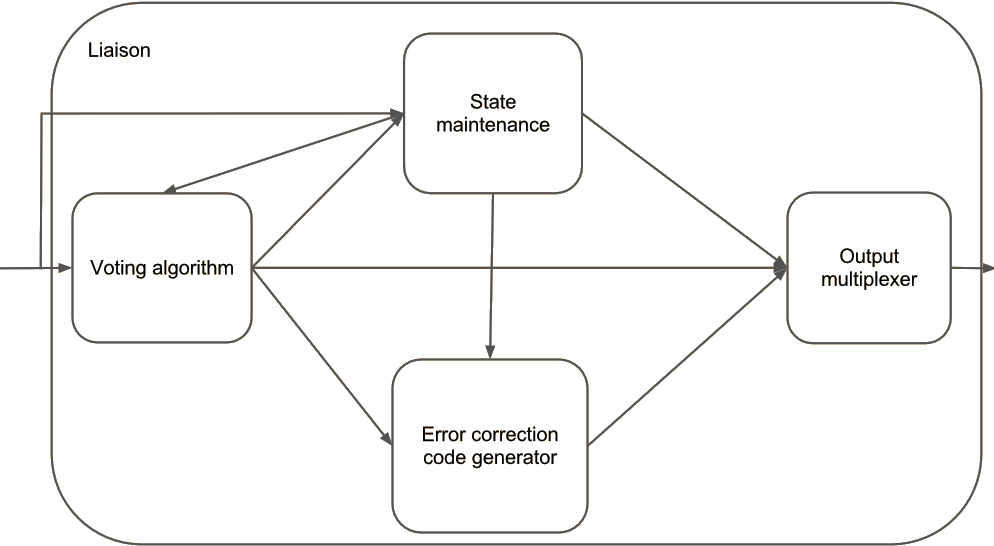
\includegraphics[width=15cm]{design/fig_overview}
\caption{Modules overview}
\label{fig:overview}
\end{figure}

An overview of our system design is depicted in
\autoref{fig:overview}. Conceptually, the internals of the Liaison can
be modeled as four different components, each responsible for a
certain task as indicated by their respective names.

\subsection{System Assumptions}
There are certain elements of the system behaviour and environment
that is not specified in the requirements. We have therefore done some
assumptions for our implementation.

\begin{itemize}
\item Outside of periods in which the microprocessors are supposed to
  be sending data to the Liaison\footnote{before or more than 8 cycles
    after a {\ttfamily di\_ready} signal, see \autoref{apx:liaison}},
  we assume that the microcontrollers are not necessarily driving the
  lines, and thus we cannot tag the microcontrollers.

\item We have assumed that two failing microcontrollers within the
  same clock cycle should not happen. This assumption is made since it
  is, in general, not possible to detect the simultaneous failure of
  two or more microcontrollers. For instance, if three controllers are
  left, and two of them fail and produce the wrong output, since they
  represent the majority they will be assumed to be working while the
  microcontroller that is actually producing correct results will be
  tagged as erroneous. Since there is no other distinction between the
  microcontrollers than the data they produce, it will be impossible
  to detect a difference between this situation and one in which one
  microcontroller fails. If four microcontrollers are working, and two
  fails, the system logic will therefore select two controllers for
  failure without knowing which really has failed. If this selection
  was correct, the system will continue functioning; if not, the two
  failed microcontrollers that was left as working will most likely
  shortly provide inconsitent data, and the system will be considered
  broken.

\item The requirements do not specify what data should be output when
  the system is failing. We assume that since the receiver will know
  that the system is broken, the data sequence can be whatever it
  likes. The most easy solution is therefore to output whatever the
  combinatorial circuits responsible for the voted data output, and we
  will not create any special logic to adjust the data message.

\end{itemize}


\subsection{Voting algorithm}
\label{sec:votingalgorithm}
The system needs to to vote for the majority result of working
microcontrollers, and this is the responsibility of the Voting
module. To perform this task, the voting module must know which
microcontrollers have previously shown signs of failure by producing
different non-majority output in earlier votes. The module receives
input directly from the microcontrollers, and it gets the error tags
of each microcontroller from the State Maintainance module.

The algorithm in our design works by partitioning the microcontrollers
into two pairs. For the following explanation, the microcontrollers
will be labeled A, B, C and D, and the groups in the partition will be
labeled (A, B) and (C, D).

First, each group performs what will be referred to as a local
vote. The result from this local vote is tabulated in
\autoref{tab:localvote}.

\begin{table}[htbp]
  \centering
  \caption{Local vote between microcontroller pairs}
  \begin{tabular}{|c|c|}
    \hline
    \textbf{Condition} & \textbf{Result} \\ \hline
    MCU1 and MCU2 both untagged & MCU1 data $\wedge$ MCU2-data \\ \hline
    Only MCU1 untagged & MCU1 data \\ \hline
    Only MCU2 untagged & MCU2 data \\ \hline
    Both tagged   & 0 \\ \hline
  \end{tabular}
  \label{tab:localvote}
\end{table}

The local vote gives the majority vote between the two
microcontrollers. In the case of a tie, or both microcontrollers being
tagged as erroneous, the output from the local vote is 0. 

The algorithm then proceeds by distinguishing between three different
scenarios. These scenarios are tabulated in
\autoref{tab:globalvote}. Note that there is an implicit condition in
addition to the one listed in each row that none of the conditions in
rows above it hold.

\begin{table}[htbp]
  \centering
  \caption{Final vote result}
  \begin{tabular}{|p{7cm}|c|}
    \hline
    \textbf{Condition} & \textbf{Result} \\ \hline
    A, B untagged and (A,B)-result is not a tie & (A,~B)-result \\ \hline
    Data from C and D is equal & (C,~D)-result \\ \hline
    Neither pair is safe  & (A,~B)-result $\vee$ (C,~D)-result \\ \hline
  \end{tabular}
  \label{tab:globalvote}
\end{table}

First, it checks whether both A and B are untagged and have the same
data value. If this is the case, then the output from the local vote
of (A,~B) will have two votes, which is enough to ensure either
majority or a tie no matter what the result from (C,~D) is.

If this is not the case, then either A or B is faulty, and the (A,
B)-result represents at most one vote. If the data from
microcontroller C and D is the same, then it represents two, one or
zero votes to the (C,~D)-result without providing any votes which
could strengthen the (A,~B)-result.

\begin{itemize}
\item If the (C,~D)-result represents two votes, it is the majority
  result, since the (A,~B) group can oppose it with at most one vote. 
  
\item If the (C,~D)-result represents one vote
  \begin{itemize}
  \item If the (A,~B)-result is a tie, then the (C,~D)-result will be
    the decisive vote. 
  \item If the (A,~B)-result represents one vote, then the (C,
    D)-result is either the majority result or there is a tie. In
    either case, the (C,~D)-result is a valid result from the vote.
  \item If the (C,~D)-result represents zero votes, then the system is
  \end{itemize}

\item If the (C,~D)-result represents zero votes, then the system must
  be broken since the (A,~B) result only represents at most one vote
  and as such only one microcontroller is still functioning correctly.
\end{itemize}

If the data from C and D is not the same, then neither pair of
microcontroller is guaranteed to represent the majority on its
own. The remaining possibilities are as follows

\begin{itemize}
\item If the (A,~B)-result is a tie, then its value is zero. It is
  thus safe to output this value ORed with the (C,~D)-result, which is
  the decisive vote.

\item If the (A,~B)-result represents a single vote
  \begin{itemize}
  \item If the (C,~D)-result is a tie, then by the same reason as in
    the first point (A,~B)-result $\vee$ (C,~D)-result is a valid
    voting result.

  \item If the (C,~D)-result also represents a single vote
    \begin{itemize}
    \item If the (A,~B)-result equals the (C,~D)-result, (A,~B)-result
      $\vee$ (C,~D)-result will produce this value.
    \item If the results are not equal, the vote is a tie and the
      output can be anything.
    \end{itemize}
  \end{itemize}

\item Any other condition represents a system broken state, in which
  only one or zero microcontrollers are still working. For these
  scenarios, the result from the vote does not matter.

\end{itemize}

\subsection{State maintainance}
The State Maintainance module is responsible for all internal states
of the system. The system keeps track of what microcontrollers that
can no longer be trusted. This works by tagging those microcontrollers
were the signal differs from the voted signal from the Voter
module. When a microcontroller has been tagged, the tag is not cleared
until the entire system is reset.

This module also outputs a system status vector as part of the Liaison
output. This vector has one of four states as shown in
\autoref{tab:systemstatus}.  The output status is a direct mapping
from the internal tag-vector, and works simply as a lookup table.

At last, the State Maintainance module is also responsible for
counting what output is sent at each clock tick. Since we are
outputing a serial data stream where different sections of the stream
have different sources (data, status, ECC), we need to keep track of
the position of the current data bit.



\subsection{Error Correcting Code Generator}
To provide reliable output for long distance transmission of data, the
Liaison System was required to add an error correcting code (ECC) to
its data packets. As stated in \autoref{sec:problem}, the ECC should
be able to correct one bit errors and detect two bit errors. To
fulfill the first criteria, we use a (15, 11)
Hamming-code\cite{ecc}. Since the Liaison sends eleven data bits ---
eight for the voted data and three for the status --- using four
parity bits is sufficient to provide detection and correction for one
bit errors. To be able to detect two bit errors, one can use an extra
parity bit covering all the transmitted bits, including data, status
and the four other ECC bits. This final parity bit is called
SECDED-bit, since it makes the Hamming code a Single Error Correction
Double Error Detection code\cite{ecc}. For simlicity, we will refer to
this error correction code scheme as a (16, 11) Hamming code. The
calculation of the parity bit is shown in \autoref{tab:hammingcode},
showing which data bits are covered by each parity bit.

\begin{table}[htbp]
  \centering
  \caption{Hamming Code Data Bit Coverage}
  \begin{tabular}{|c|c|c|c|c|c|c|c|c|c|c|c|c|c|c|c|c|}
    \hline
   & d0 & d1 & d2 & d3 & d4 & d5 & d6 & d7 & d8 & d9 & d10 & p0 & p1 & p2 & p3 & p4 \\ \hline
p0 & X  & X  &    & X  & X  &    & X  &    & X  &    & X   & X  &    &    &    &    \\ \hline
p1 & X  &    & X  & X  &    & X  & X  &    &    & X  & X   &    & X  &    &    &    \\ \hline
p2 &    & X  & X  & X  &    &    &    & X  & X  & X  & X   &    &    & X  &    &    \\ \hline
p3 &    &    &    &    & X  & X  & X  & X  & X  & X  & X   &    &    &    & X  &    \\ \hline
p4 & X  & X  & X  & X  & X  & X  & X  & X  & X  & X  & X   & X  & X  & X  & X  & X  \\ \hline
    
  \end{tabular}
  \label{tab:hammingcode}
\end{table}


The Error Correcting Code Generator generates (16,11) Hamming code on
the fly and attaches the code at the end of the output stream. This
module uses information from the Voter to get the first eight data
bits and information from the State Maintainance to get the status
word. It also uses information of current data bit position from the
State Maintainance module, since Hamming Code is generated using
parity of bits at specific positions\cite{ecc}.

\subsection{Output Multiplexer}
Since the Liaison System needs to send output from each of the three other modules at specific clock cycles when specific events has occured, we need
a logic piece of hardware that can multiplex all modules and allways output the correct signal. The Output Multiplexer uses the position of current data bit
from the State Maintainance module to select what module to send data from.
